\section{Risultati}
\label{sec:risultati}

In questa sezione verranno presentati i risultati degli esperimenti sulle varie euristiche. Gli esperimenti sono stati eseguiti su un totale di 40 problemi diversi. 

Per valutare le euristiche, sono state utilizzate diverse metriche:

\begin{itemize}
\item \textbf{Media passi}: la media del numero di passi necessari per chiudere il problema, calcolata su tutti i problemi;
\item \textbf{Media fissati}: la media di nodi fissati ad ogni iterazione, calcolata su tutte le iterazioni di tutti i problemi;
\item \textbf{Media max nodi fissati}: per ogni problema, viene calcolato il numero di nodi fissati ad ogni iterazione. Viene preso il numero di nodi fissati dell'iterazione che ne ha fissati di più per ogni problema, e viene effettuata la media di tale valore su ogni problema;
\item \textbf{Media nodi no fissati:} la media del numero di iterazioni in cui non vengono fissati nodi, calcolata considerando tutte le iterazioni di tutti i problemi;
\item \textbf{Max passi}: numero di passi necessari per chiudere il problema che ha richiesto più iterazioni;
\item \textbf{Max max nodi fissati}: numero massimo di nodi fissati in un passo, calcolato considerando ogni iterazione di ogni problema;
\item \textbf{Min nodi no fissati}: minimo numero di iterazioni in cui non sono stati fissati nodi, calcolato su tutte le iterazioni di tutti i problemi.
\end{itemize}

La Tabella \ref{tab:results} mostra i risultati delle euristiche proposte sulle metriche presentate sopra. I migliori risultati per ogni metrica sono evidenziati in grassetto. 

\begin{sidewaystable}[htbp]
\centering
\begin{tabular}{l|c|c|c|c|c|c|c|c}
\rowcolor[HTML]{EFEFEF} 
\textbf{Euristica}  & \textbf{Media passi} & \textbf{\begin{tabular}[c]{@{}c@{}}Media\\ fissati\end{tabular}} & \textbf{\begin{tabular}[c]{@{}c@{}}Media\\ max nodi\\ fissati\end{tabular}} & \textbf{\begin{tabular}[c]{@{}c@{}}Media\\ nodi\\ no fissati\end{tabular}} & \textbf{Max passi} & \textbf{\begin{tabular}[c]{@{}c@{}}Max\\ fissati\end{tabular}} & \textbf{\begin{tabular}[c]{@{}c@{}}Max max\\ nodi fissati\end{tabular}} & \textbf{\begin{tabular}[c]{@{}c@{}}Min nodi\\ no fissati\end{tabular}} \\ \hline
aux                 & 1791.4               & 3.1335912648                                                     & \textit{272.8}                                                              & 14592.2                                                                    & 9298               & 3.6839212093                                                   & \textit{283}                                                            & 429                                                                    \\ \hline
\rowcolor[HTML]{EFEFEF} 
auxMaxPeso          & 341.45               & 21.5602317507                                                    & 585                                                                         & 1407.15                                                                    & 1313               & 34.3806228374                                                  & 613                                                                     & 27                                                                     \\ \hline
auxMinPeso          & 2810.35              & 1.5978815539                                                     & 569.6                                                                       & 27715.55                                                                   & 14024              & 2.0287322275                                                   & 608                                                                     & 895                                                                    \\ \hline
\rowcolor[HTML]{EFEFEF} 
maxArchiDaFissare   & 243.2                & 31.0389286082                                                    & 328.45                                                                      & \textbf{0}                                                                 & 1246               & 36.8441558442                                                  & 405                                                                     & \textbf{0}                                                             \\ \hline
maxPeso             & \textbf{188.55}      & \textbf{37.2322594837}                                           & \textbf{604.7}                                                              & \textbf{0}                                                                 & \textbf{938}       & \textbf{50.125}                                                & 651                                                                     & \textbf{0}                                                             \\ \hline
\rowcolor[HTML]{EFEFEF} 
minArchiDaFissare   & \textit{2882.75}     & \textit{1.529461278}                                             & 354.9                                                                       & \textit{28413.85}                                                          & \textit{14225}     & \textit{2.0233589592}                                          & 393                                                                     & \textit{934}                                                           \\ \hline
minPeso             & 608.9                & 12.2729528981                                                    & 354.6                                                                       & 1656.8                                                                     & 3262               & 17.2156862745                                                  & 468                                                                     & 54                                                                     \\ \hline
\rowcolor[HTML]{EFEFEF} 
noAuxNoThorn        & 498.15               & 16.4752997265                                                    & 314                                                                         & 4.15                                                                       & 2637               & 24.5614035088                                                  & 372                                                                     & \textbf{0}                                                             \\ \hline
noAuxNoThornMaxPeso & \textbf{188.55}      & \textbf{37.2322594837}                                           & \textbf{604.7}                                                              & \textbf{0}                                                                 & \textbf{938}       & \textbf{50.125}                                                & 651                                                                     & \textbf{0}                                                             \\ \hline
\rowcolor[HTML]{EFEFEF} 
noAuxNoThornMinPeso & 358.1                & 20.4006207465                                                    & 585.2                                                                       & 113.35                                                                     & 1809               & 25.2179487179                                                  & 683                                                                     & 5                                                                      \\ \hline
thorn               & 562.55               & 12.0982982476                                                    & 567.95                                                                      & 3251.9                                                                     & 2608               & 15.762295082                                                   & 646                                                                     & 125                                                                    \\ \hline
\rowcolor[HTML]{EFEFEF} 
thornMaxPeso        & 332.15               & 21.485487372                                                     & 584.45                                                                      & 1089.85                                                                    & 1236               & 38.4787644788                                                  & \textbf{921}                                                            & 31                                                                     \\ \hline
thornMinPeso        & 728.6                & 8.9800927173                                                     & 601.35                                                                      & 5384.8                                                                     & 3400               & 12.3660130719                                                  & 644                                                                     & 199                                                                   
\end{tabular}
\caption{Risultati delle euristiche sulle diverse metriche.}
\label{tab:results}
\end{sidewaystable}

Come si può vedere, l'euristica \textit{noAuxNoThornMaxPeso}, insieme all'euristica \textit{maxPeso}, sono quelle che, generalmente, portano ai migliori risultati. Non solo: i risultati di entrambe le euristiche sono gli stessi su ogni metrica. Questo significa che l'euristica \textit{maxPeso}, che favorisce i nodi a cui è assegnato peso maggiore, sembra essere la migliore per i problemi considerati, ma che prendere in considerazione la classe del nodo oltre al suo peso non porta alcuna variazione nei risultati.

Invece, l'euristica che nel complesso sembra avere il comportamento peggiore è \textit{minArchiDaFissare}, portando ai peggiori risultati su 5 delle 7 metriche testate. Nelle restanti due metriche (\textit{media max nodi fissati} e \textit{max max nodi fissati}), l'euristica \textit{minArchiDaFissare} è comunque fra le peggiori.

La discussione si concentrerà ora nel dettaglio delle varie metriche, analizzandone i risultati delle diverse euristiche.

\subsection{Media passi}
\label{subsec:mediaPassi}
I risultati delle varie euristica sulla metrica \textit{media passi} sono mostrate graficamente in Figura \ref{fig:mediaPassi}.

\begin{figure}[H]
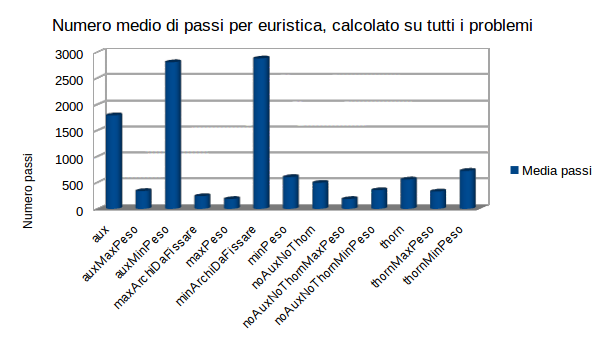
\includegraphics[width=\textwidth]{res/img/mediaPassi.png}
\caption{Rappresentazione grafica dei risultati della varie euristiche sulla metrica \textit{media passi}.}
\label{fig:mediaPassi}
\end{figure}

Per quanto riguarda il numero di passi necessari a chiudere il problema, la maggior parte delle euristiche testate si comporta piuttosto bene, rimandendo al di sotto degli 800 passi. Tuttavia, le tre euristiche \textit{aux}, \textit{auxMinPeso} e \textit{minArchiDaFissare} necessitano di molti più passi (circa 1800 la prima, sopra i 2500 le seconde) per chiudere il problema.

\subsection{Media fissati}
I risultati delle varie euristica sulla metrica \textit{media fissati} sono mostrate graficamente in Figura \ref{fig:mediaFissati}.

\begin{figure}[H]
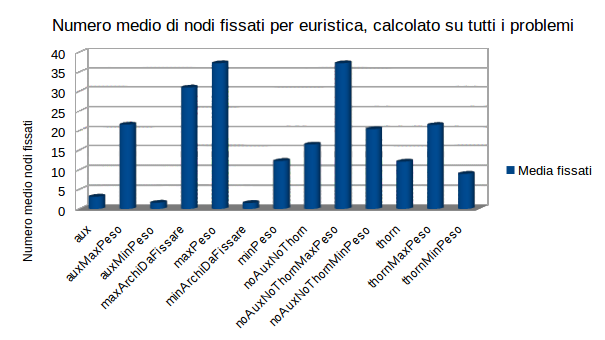
\includegraphics[width=\textwidth]{res/img/nodiFissati.png}
\caption{Rappresentazione grafica dei risultati della varie euristiche sulla metrica \textit{media fissati}.}
\label{fig:mediaFissati}
\end{figure}

La metrica \textit{media fissati} definisce il numero medio di nodi fissati sulle diverse iterazioni nei vari problemi. Come accennato precedentemente, le euristiche \textit{maxPeso} e \textit{noAuxNoThornMaxPeso} fissano mediamente il maggior numero di nodi (in media, 37 ad iterazione). Anche l'euristica \textit{maxArchiDaFissare} si comporta piuttosto bene, fissando mediamente 31 nodi ad iterazione. Invece, le euristiche \textit{aux}, \textit{auxMinPeso} e \textit{minArchiDaFissare} riescono a fissare meno di 5 nodi ad iterazione: conseguentemente, il numero di passi per chiudere il problema aumenta, come visto in Sezione \ref{subsec:mediaPassi}.

\subsection{Media max nodi fissati}
I risultati delle varie euristica sulla metrica \textit{media max nodi fissati} sono mostrate graficamente in Figura \ref{fig:mediaMaxNodiFissati}.

\begin{figure}[H]
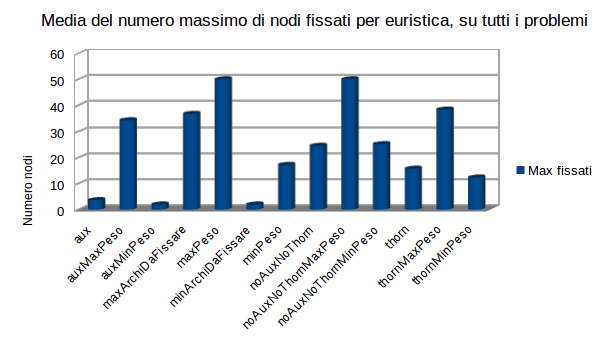
\includegraphics[width=\textwidth]{res/img/mediaMaxFissati.png}
\caption{Rappresentazione grafica dei risultati della varie euristiche sulla metrica \textit{media max nodi fissati}.}
\label{fig:mediaMaxNodiFissati}
\end{figure}

Questa metrica riconferma la qualità delle euristiche \textit{maxPeso} e \textit{noAuxNoThornMaxPeso} e la inefficacia delle euristiche \textit{aux}, \textit{auxMinPeso} e \textit{minArchiDaFissare}. Possiamo inoltre notare che le euristiche \textit{auxMaxPeso}, \textit{maxArchiDaFissare} e \textit{thornMaxPeso} ottengono buoni risultati.

\subsection{Media nodi non fissati}
I risultati delle varie euristica sulla metrica \textit{media nodi no fissati} sono mostrate graficamente in Figura \ref{fig:mediaNodiNoFissati}.

\begin{figure}[H]
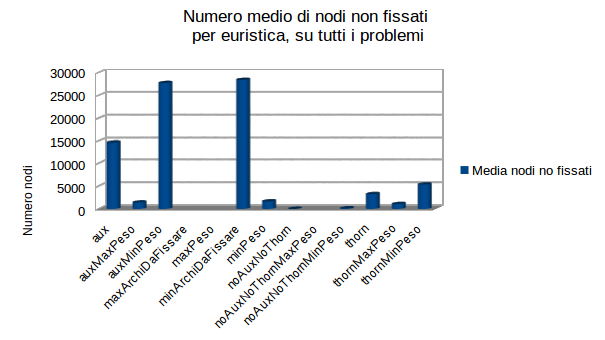
\includegraphics[width=\textwidth]{res/img/mediaNodiNoFissati.png}
\caption{Rappresentazione grafica dei risultati della varie euristiche sulla metrica \textit{media nodi no fissati}.}
\label{fig:mediaNodiNoFissati}
\end{figure}

Questa metrica riflette il numero di iterazioni in cui la riduzione non riesce a fissare nessun nodo. Perciò, un buon approccio euristico dovrebbe minimizzare questo numero. In generale, le varie euristiche hanno ottenuto buoni risultati su questa metrico, eccetto per \textit{aux}, \textit{auxMinPeso} e \textit{minArchiDaFissare}.

\subsection{Max passi}
I risultati delle varie euristica sulla metrica \textit{max passi} sono mostrate graficamente in Figura \ref{fig:maxPassi}.

\begin{figure}[H]
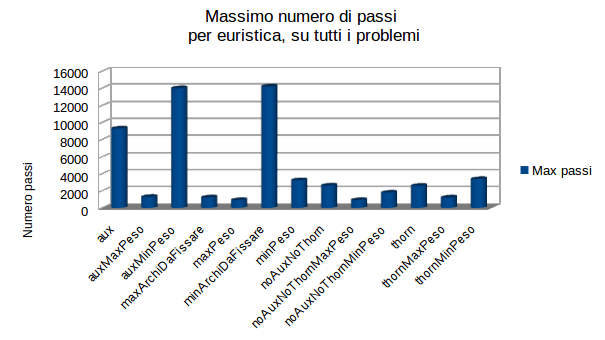
\includegraphics[width=\textwidth]{res/img/maxPassi.png}
\caption{Rappresentazione grafica dei risultati della varie euristiche sulla metrica \textit{max passi}.}
\label{fig:maxPassi}
\end{figure}

Questa metrica riconferma le considerazione fatte in precedenza senza aggiungere particolari informazioni interessanti. Anche qui, le varie euristiche hanno buoni risultati eccetto \textit{aux}, \textit{auxMinPeso} e \textit{minArchiDaFissare}.

\subsection{Max max nodi fissati}
I risultati delle varie euristica sulla metrica \textit{max max nodi fissati} sono mostrate graficamente in Figura \ref{fig:maxMaxNodiFissati}.

\begin{figure}[H]
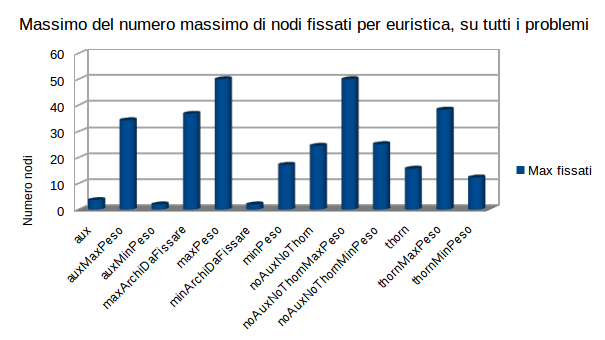
\includegraphics[width=\textwidth]{res/img/maxMaxNodiFissati.png}
\caption{Rappresentazione grafica dei risultati della varie euristiche sulla metrica \textit{max max nodi fissati}.}
\label{fig:maxMaxNodiFissati}
\end{figure}

Questa metrica mostra risultati interessanti. Infatti, possiamo vedere come in questo caso l'euristica \textit{maxPeso}, con un numero massimo assoluto di nodi fissati di 651, non sia più la migliore, sebbene rimanga comunque fra le migliori euristiche. Invece, l'euristica \textit{thornMaxPeso} risulta essere la migliore, con un numero massimo di nodi fissati di 931. Questo significa che tale euristica, in un determinato problema, ha fissato 931 nodi in una sola iterazione. Potrebbe essere quindi interessante capire se questa euristica possa essere particolarmente performante su una specifica classe di problemi.

\subsection{Min nodi no fissati}
I risultati delle varie euristica sulla metrica \textit{min nodi no fissati} sono mostrate graficamente in Figura \ref{fig:minNodiNoFissati}.

\begin{figure}[H]
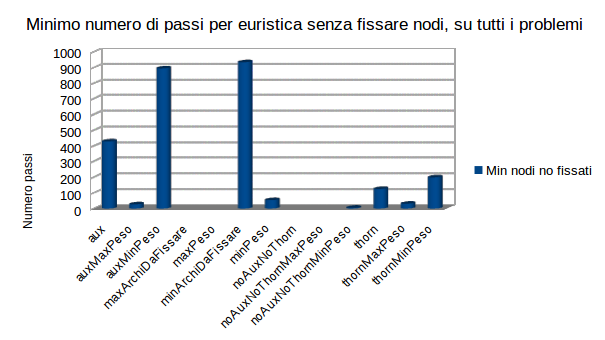
\includegraphics[width=\textwidth]{res/img/minNodiNoFissati.png}
\caption{Rappresentazione grafica dei risultati della varie euristiche sulla metrica \textit{min nodi no fissati}.}
\label{fig:minNodiNoFissati}
\end{figure}

Anche questa metrica riconferma le considerazioni fatte in precedenza: \textit{aux}, \textit{auxMinPeso} e \textit{minArchiDaFissare} danno risultati particolarmente negativi, mentre le altre euristiche hanno risultati generalmente buoni. 